\documentclass{standalone}
\usepackage{tikz}
\usepackage{ctex,siunitx}
\usepackage{tkz-euclide}
\usepackage{amsmath}
\usetikzlibrary{patterns, calc}
\usetikzlibrary {decorations.pathmorphing, decorations.pathreplacing, decorations.shapes,}
\begin{document}
\small
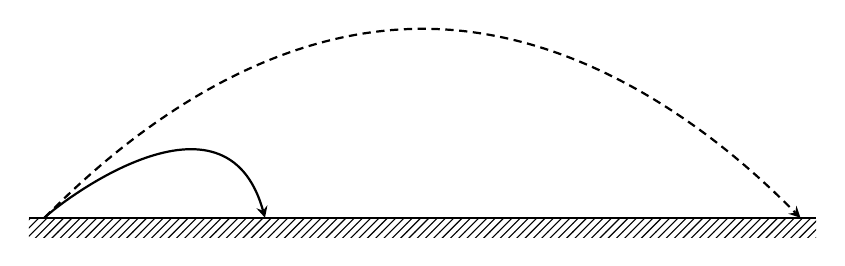
\begin{tikzpicture}[>=stealth,scale=1]
  % \useasboundingbox (-0.1,0.1) rectangle(6.1,-3.1);
  \draw[thick](-5,0)--(5,0);
  \fill[pattern = north east lines] (-5,0)rectangle(5,-0.25);
  \draw[thick,->,densely dashed] (-4.8,0) parabola [bend pos =0.5] bend (0,2.4) (4.8,0);
  % \draw[thick] (-1.5,1.5) parabola (-4.8,0);
  \draw [thick,->] (-4.8,0)..controls(-4.6,.2)and(-2.5,1.8)..(-2.0,0);
\end{tikzpicture}
\end{document}